% CHAPTER 1
\chapter{POWER SYSTEM FREQUENCY STABILITY}
\label{chp:2}
\section{Synchronous Generator and Synchronous Speed}

Synchronous machines produce torque only in synchronous speed. This is why they are equipped with damper windings which are basically induction machine windings. If the frequency of  grid changes, damper windings create a torque which creates a force to synchronize the speed to the grid frequency. Two type of damper windings are given in Fig. \ref{damperwindings}.

\begin{figure}[h!]
	\centering
	\begin{subfigure}{.5\textwidth}
		\centering
		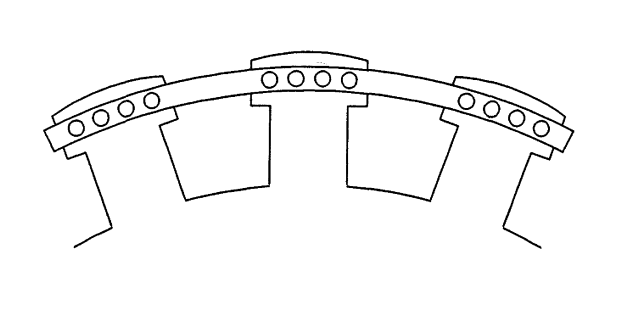
\includegraphics[width=.95\linewidth]{continuousdamper.png}
		\caption{continuous damper}
		\label{continuousdamper}
	\end{subfigure}%
	\begin{subfigure}{.5\textwidth}
		\centering
		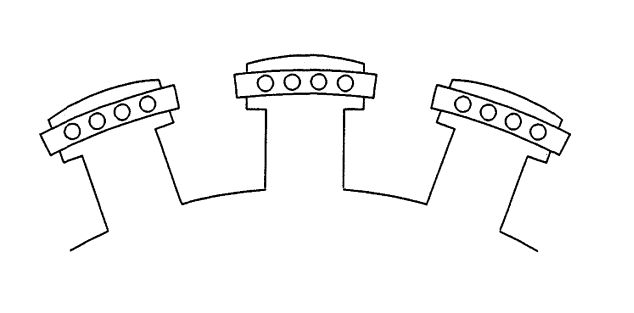
\includegraphics[width=.95\linewidth]{noncontinuousdamper.png}
		\caption{non-continuous damper}
		\label{noncontinuousdamper}
	\end{subfigure}
	\caption{Damper windings in a synchronous generator \cite{Kundur}}
	\label{damperwindings}
\end{figure}

The synchronous machines keep their operation in the synchronous speed thanks to the damper windings in the rotor. Relation between grid frequency and the synchronous speed is given in Eq. (\ref{syncspeed}) in terms of rpm. \cite{Kundur}. This equation can be better observed in Eq (\ref{syncspeed2}).

\begin{equation}
 n_{s}=\frac{120f}{p_{f}}
 \label{syncspeed}
\end{equation}
\begin{equation}
 n_{s}=\frac{60}{2\pi}\omega_{syn}
\end{equation}
\begin{equation}
\omega_{syn}=\frac{4\pi f}{p_{f}}
\label{syncspeed2}
\end{equation}

where $n_{s}$ is the synchronous speed in rpm, $f$ is the grid frequency in Hz, $p_{f}$ is the number of poles of the generator and $\omega_{syn}$ is the synchronous angular speed in rad/s.

\section{Swing Equation}
\label{swing}
Speed in synchronous machines changes according to the net torque acting on the rotor. Therefore, the speed is maintained constant unless there is no difference between mechanical and electromechanical torque. The equation of motion is given in Eq. (\ref{eqmotion}) where $J$ is aggravated moment of inertia of the generator and the turbine in $kgm^{2}$,$T_{m}$ and $T_{e}$ are mechanical and electromechanical torques in $Nm$.
\begin{equation}
J\frac{d\omega_{m}}{dt}=T_{m}-T_{e}=T_{a}
\label{eqmotion}
\end{equation}
In power system network, the power ratings of the generators and corresponding moment of inertia values varies. Hence, it is more convenient to use inertia constant, $H$ whose unit is seconds and varies between 2 and 9 \cite{Kundur}. Inertia constant is defined as the ratio of kinetic energy stored in the inertia to the power rating of the generator as in Eq. (\ref{inertiaconstant}) where $\omega_{0m}$ denotes the rated angular velocity of generator in rad/s and $S_{base}$ is the rated apparent power in VA. 
\begin{equation}
H=\frac{{\frac{1}{2}}J\omega_{0m}^{2}}{S_{base}}
\label{inertiaconstant}
\end{equation}

Substituting Eq. (\ref{inertiaconstant}) into Eq. (\ref{eqmotion}) and replacing units to per-unit quantities yield the relation of frequency with power and inertia constant as in Eq. (\ref{eqmotion5}).
\begin{equation}
J=\frac{2H}{\omega_{0m}^{2}}{S_{base}}
\label{inertiaconstant2}
\end{equation}
\begin{equation}
\frac{2H}{\omega_{0m}^{2}}{S_{base}}\frac{d\omega_{m}}{dt}=T_{m}-T_{e}
\label{eqmotion2}
\end{equation}
\begin{equation}
\frac{2H}{\omega_{0m}^{2}}{S_{base}\omega_{m}}\frac{d\omega_{m}}{dt}=P_{m}-P_{e}
\label{eqmotion3}
\end{equation}
\begin{equation}
2H\frac{\omega_{m}}{\omega_{0m}}\frac{d(\omega_{m}/\omega_{0m})}{dt}=\frac{P_{m}-P_{e}}{S_{base}}
\label{eqmotion4}
\end{equation}
\begin{equation}
2H\overline{\omega_{m}}\frac{d\overline{\omega_{m}}}{dt}=\overline{P_{m}}-\overline{P_{e}}
\label{eqmotion5}
\end{equation}
\section{Frequency in Power Systems}
The frequency in a power system is related to the speed of the synchronous generators and changes according to the swing equation. The frequency of the each generator is not the same in the network since each generator does not have the same speed. There are always fluctuations in the power system. However, the network can be assumed as a single generating unit by neglecting this assumption. The swing equation basically investigates the relation between mechanical and electromechanical powers and the rate of change of angular speed of a generator. Therefore, the speed of an generator remains constant if the mechanical and electromechanical powers are equal.\\
If the electricity grid is considered as a single generator, the inertia of the equivalent generator is aggravated from each generator in the network. In this case, average frequency in the network can be found as in Eq. (\ref{systemswing})
\begin{equation}
\label{systemswing}
2H_{sys}\overline{f_{sys}}\frac{d\overline{f_{sys}}}{dt}=\overline{P_{m}}-\overline{P_{e}}
\end{equation}
where $P_{m}$ is the aggravated mechanical input power of the generators meanwhile $P_{e}$ is the aggravated electromechanical output power. In other words, the system frequency depends on the balance between generation and consumption. Note that generation means the input mechanical power of the generators.\par
\begin{figure}[h!]
	\centering
	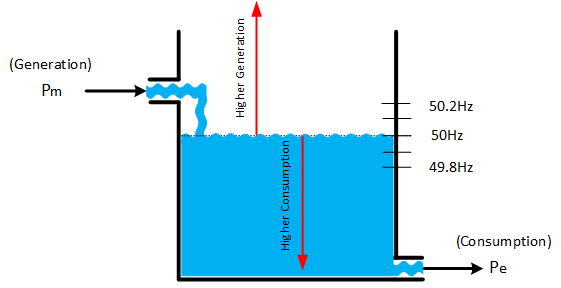
\includegraphics[width=.95\linewidth]{frequencypool.png}
	\caption{Frequency behaviour in electric grid with the water level in a container analogy \cite{Eto2010}}
	\label{frequencyingrid}
\end{figure}
The behaviour of the frequency in electric grid is depicted in Fig. \ref{frequencyingrid}. As it can be seen from the water level in a container analogy, the frequency of the system is dependent on the in-flow and the out-flow. Therefore, in the electricity grid, frequency increases as the aggravated input power is higher than the aggravated output power. Note that, the direction of the frequency is dictated by this balance. Having a constant 49.8Hz frequency does not mean that consumption is higher than generation. If the frequency is constant, then the input mechanical power is equal to output power.
\subsection{Primary Frequency Control}
Having a constant frequency is one of the most important responsibilities of a system operator. In order to have a constant frequency, supply is being adjusted according to the demand continuously. By doing so, the system frequency varies between a band-gap. The variation depends on the disturbances which are generally a sudden generation outage or instant load connection. The size of the disturbance determines the severity of the frequency change and there are three main mechanisms to arrest the frequency changes in the system. \\
Following generator outage or sudden load connection event, frequency start decreasing. The slope of the frequency is dependent on the severity of the event by means of power and the available inertia of the power system. Such frequency disturbance requires increased input power. However, the increase in the input mechanical power should be activated very fast and should be automated. This responsibility is assigned to generating units with primary control. The active power generation of these units is increased or decreased by the governor depending on the network frequency direction. Note that each generator in the power system does not necessarily perform primary control function. In this case, their active power generation is independent from the network frequency. Hence, the decrease in the frequency is arrested by the primary frequency control. The primary controllers act during a few seconds following a disturbance. They keep their operation up to 30 minutes. 
\subsection{Secondary and Tertiary Control}
The frequency is recovered back to nominal value with the Secondary Frequency Control action. This controller might be a single or multiple centres that monitor the frequency and adjust the generation accordingly. They are also called as Automatic Generation Control (AGC) systems and their action takes a few minutes. The final frequency control mechanism is the Tertiary Frequency Control. If the frequency is not recovered back to nominal value with the secondary controllers, tertiary frequency controllers manually activates the load shedding which is an undesired situation by the network operator. However, it is an emergency case which might result in black-out and requires immediate action.
\section{Energy Market}
The frequency is kept inside the operational band in the electricity network by balancing the supply and the demand by intersecting the supply and demand curves inside the different time intervals. In this way, the balance is ensured in the market by day ahead, intra-day and balancing markets. 
\subsection{Day Ahead Market}
The load power in a network has a distinct characteristic depending on the day of the week or the hour of the day. By foreseeing the next day demand power variation, the electricity market collects the bids from the energy suppliers and consumers. According to submitted bids, the next day generation price is determined by intersecting the supply and demand price curves. The price of the energy is called Market Clearing Price (MCP). These bids are submitted for the next day and the prices are determined before the corresponding day.
\subsection{Intra-Day Market}
Even though the estimations for the upcoming day load power has superior accuracy with the advanced estimation methods, networks are subjected to unexpected problems such as generator trips, line outages. Therefore, intra-day market contributes the balance of the market between the day ahead market and balancing market. Moreover, it gives the participants almost real-time trading opportunity meanwhile it increases the sustainability of the market. After day ahead market has closed for the corresponding day, the bids are submitted to system. In other words, MCP is already determined for the corresponding day meanwhile the rest of the day prices are not set. 
\subsection{Balancing Market}
Primary and secondary control reserves are maintained in the system in order to improve the balance for the instant deviations in the frequency. The frequency is first arrested by the primary controllers and it is restored by the secondary controllers. The generation units that participate primary and secondary control promises a defined generation capacity to these actions. Balancing market is much more different than day ahead and intra-day market since its main goal is the network security rather than electricity trading. The price of the energy in this market called as System Marginal Price (SMP).
\subsection{Electricity Price for Renewable Energy Systems}
The main source of the significant energy produced in the Turkish electricity network is exported. As a result of this, the energy sector is highly dependent on the foreign countries. In order to decrease the dependency on the external sources, the renewable energy sources are supported by government in Turkey. The energy generated by renewable energy systems are bought with feed-in tariff (FIT) with a pre-determined time period. This decreases the return of investment due to the fact that all produced energy will be bought during this period. The feed-in tariff for different renewable energy systems is listed in Table \ref{price} \cite{yasa}.\par
\begin{table}[h]
	\centering
	\begin{tabular}{cc}
		\hline
		\textbf{Renewable Energy System} & \textbf{\begin{tabular}[c]{@{}c@{}}Feed-In Tariff\\ (cent/kWh)\end{tabular}} \\ \hline
		Hydro                            & 7.3                                                                          \\
		Wind                             & 7.3                                                                          \\
		Geothermal                       & 10.5                                                                         \\
		Biomass                          & 13.3                                                                         \\
		Solar                            & 13.3                                                                         \\ \hline
	\end{tabular}
\caption{Feed-In Tariff for Renewable Energy Systems in Turkey}
\label{price}
\end{table}
In addition to feed-in tariff, energy provider can benefit from additional incentives as long as some parts of the system is produced inside Turkey. For instance, by preferring the tower of a wind turbine which is a domestic production, an additional price is given to energy provider as local-bonus content. The local-bonus contents for wind turbines are listed in Table \ref{price2} \cite{yasa}.

\begin{table}[h!]
	\centering
	\begin{tabular}{cc}
		\hline
		\textbf{\begin{tabular}[c]{@{}c@{}}Local Content\\ for Wind Turbines\end{tabular}}   & \textbf{\begin{tabular}[c]{@{}c@{}}Local Content Incentive\\ (cent/kWh)\end{tabular}} \\ \hline
		Blade                                                                                & 0.8                                                                                   \\
		\begin{tabular}[c]{@{}c@{}}Generator and \\ Power Electronics\end{tabular}           & 1.0                                                                                   \\
		Turbine Tower                                                                        & 0.6                                                                                   \\
		\begin{tabular}[c]{@{}c@{}}All mechanical parts in \\ Rotor and Nacelle\end{tabular} & 1.3                                                                                   \\ \hline
	\end{tabular}
	\caption{Local Content Incentives for Wind Turbines}
	\label{price2}
\end{table}